%%%%%%%%%%%%%%%%%%%%%%%%%%%%%%%%%%%%%%%%%
% Programming/Coding Assignment
% LaTeX Template
%
% This template has been downloaded from:
% http://www.latextemplates.com
%
% Original author:
% Ted Pavlic (http://www.tedpavlic.com)
%
% Note:
% The \lipsum[#] commands throughout this template generate dummy text
% to fill the template out. These commands should all be removed when 
% writing assignment content.
%
% This template uses a Perl script as an example snippet of code, most other
% languages are also usable. Configure them in the "CODE INCLUSION 
% CONFIGURATION" section.
%
%%%%%%%%%%%%%%%%%%%%%%%%%%%%%%%%%%%%%%%%%

%----------------------------------------------------------------------------------------
%	PACKAGES AND OTHER DOCUMENT CONFIGURATIONS
%----------------------------------------------------------------------------------------

\documentclass{article}

\usepackage{fancyhdr} % Required for custom headers
\usepackage{lastpage} % Required to determine the last page for the footer
\usepackage{extramarks} % Required for headers and footers
\usepackage[usenames,dvipsnames]{color} % Required for custom colors
\usepackage{graphicx} % Required to insert images
\usepackage{subcaption}
\usepackage{listings} % Required for insertion of code
\usepackage{courier} % Required for the courier font
\usepackage{lipsum} % Used for inserting dummy 'Lorem ipsum' text into the template

% Margins
\topmargin=-0.45in
\evensidemargin=0in
\oddsidemargin=0in
\textwidth=6.5in
\textheight=9.0in
\headsep=0.25in

\linespread{1.1} % Line spacing

% Set up the header and footer
\pagestyle{fancy}
\lhead{\hmwkAuthorName} % Top left header
\chead{\hmwkClass\ (\hmwkClassTime): \hmwkTitle} % Top center head
%\rhead{\firstxmark} % Top right header
\lfoot{\lastxmark} % Bottom left footer
\cfoot{} % Bottom center footer
\rfoot{Page\ \thepage\ of\ \protect\pageref{LastPage}} % Bottom right footer
\renewcommand\headrulewidth{0.4pt} % Size of the header rule
\renewcommand\footrulewidth{0.4pt} % Size of the footer rule

\setlength\parindent{0pt} % Removes all indentation from paragraphs

%----------------------------------------------------------------------------------------
%	CODE INCLUSION CONFIGURATION
%----------------------------------------------------------------------------------------

\definecolor{MyDarkGreen}{rgb}{0.0,0.4,0.0} % This is the color used for comments
\lstloadlanguages{Perl} % Load Perl syntax for listings, for a list of other languages supported see: ftp://ftp.tex.ac.uk/tex-archive/macros/latex/contrib/listings/listings.pdf
\lstset{language=Perl, % Use Perl in this example
        frame=single, % Single frame around code
        basicstyle=\small\ttfamily, % Use small true type font
        keywordstyle=[1]\color{Blue}\bf, % Perl functions bold and blue
        keywordstyle=[2]\color{Purple}, % Perl function arguments purple
        keywordstyle=[3]\color{Blue}\underbar, % Custom functions underlined and blue
        identifierstyle=, % Nothing special about identifiers                                         
        commentstyle=\usefont{T1}{pcr}{m}{sl}\color{MyDarkGreen}\small, % Comments small dark green courier font
        stringstyle=\color{Purple}, % Strings are purple
        showstringspaces=false, % Don't put marks in string spaces
        tabsize=5, % 5 spaces per tab
        %
        % Put standard Perl functions not included in the default language here
        morekeywords={rand},
        %
        % Put Perl function parameters here
        morekeywords=[2]{on, off, interp},
        %
        % Put user defined functions here
        morekeywords=[3]{test},
       	%
        morecomment=[l][\color{Blue}]{...}, % Line continuation (...) like blue comment
        numbers=left, % Line numbers on left
        firstnumber=1, % Line numbers start with line 1
        numberstyle=\tiny\color{Blue}, % Line numbers are blue and small
        stepnumber=5 % Line numbers go in steps of 5
}

% Creates a new command to include a perl script, the first parameter is the filename of the script (without .pl), the second parameter is the caption
\newcommand{\perlscript}[2]{
\begin{itemize}
\item[]\lstinputlisting[caption=#2,label=#1]{#1.pl}
\end{itemize}
}

%----------------------------------------------------------------------------------------
%	DOCUMENT STRUCTURE COMMANDS
%	Skip this unless you know what you're doing
%----------------------------------------------------------------------------------------

% Header and footer for when a page split occurs within a problem environment
\newcommand{\enterProblemHeader}[1]{
%\nobreak\extramarks{#1}{#1 continued on next page\ldots}\nobreak
%\nobreak\extramarks{#1 (continued)}{#1 continued on next page\ldots}\nobreak
}

% Header and footer for when a page split occurs between problem environments
\newcommand{\exitProblemHeader}[1]{
%\nobreak\extramarks{#1 (continued)}{#1 continued on next page\ldots}\nobreak
%\nobreak\extramarks{#1}{}\nobreak
}

\setcounter{secnumdepth}{0} % Removes default section numbers
\newcounter{homeworkProblemCounter} % Creates a counter to keep track of the number of problems
\setcounter{homeworkProblemCounter}{-1}

\newcommand{\homeworkProblemName}{}
\newenvironment{homeworkProblem}[1][Problem \arabic{homeworkProblemCounter}]{ % Makes a new environment called homeworkProblem which takes 1 argument (custom name) but the default is "Problem #"
\stepcounter{homeworkProblemCounter} % Increase counter for number of problems
\renewcommand{\homeworkProblemName}{#1} % Assign \homeworkProblemName the name of the problem
\section{\homeworkProblemName} % Make a section in the document with the custom problem count
\enterProblemHeader{\homeworkProblemName} % Header and footer within the environment
}{
\exitProblemHeader{\homeworkProblemName} % Header and footer after the environment
}

\newcommand{\problemAnswer}[1]{ % Defines the problem answer command with the content as the only argument
\noindent\framebox[\columnwidth][c]{\begin{minipage}{0.98\columnwidth}#1\end{minipage}} % Makes the box around the problem answer and puts the content inside
}

\newcommand{\homeworkSectionName}{}
\newenvironment{homeworkSection}[1]{ % New environment for sections within homework problems, takes 1 argument - the name of the section
\renewcommand{\homeworkSectionName}{#1} % Assign \homeworkSectionName to the name of the section from the environment argument
\subsection{\homeworkSectionName} % Make a subsection with the custom name of the subsection
\enterProblemHeader{\homeworkProblemName\ [\homeworkSectionName]} % Header and footer within the environment
}{
\enterProblemHeader{\homeworkProblemName} % Header and footer after the environment
}

%----------------------------------------------------------------------------------------
%	NAME AND CLASS SECTION
%----------------------------------------------------------------------------------------

\newcommand{\hmwkTitle}{Assignment\ \#$\sqrt{-1}$} % Assignment title
\newcommand{\hmwkDueDate}{Friday,\ January\ 1,\ 2016} % Due date
\newcommand{\hmwkClass}{CSC320} % Course/class
\newcommand{\hmwkClassTime}{L0101} % Class/lecture time
\newcommand{\hmwkAuthorName}{Firstname Lastname} % Your name

%----------------------------------------------------------------------------------------
%	TITLE PAGE
%----------------------------------------------------------------------------------------

\title{
\vspace{2in}
\textmd{\textbf{\hmwkClass:\ \hmwkTitle}}\\
\normalsize\vspace{0.1in}\small{Due\ on\ \hmwkDueDate}\\
\vspace{0.1in}
\vspace{3in}
}

\author{\textbf{\hmwkAuthorName}}
%\date{} % Insert date here if you want it to appear below your name

%----------------------------------------------------------------------------------------

\begin{document}

\maketitle
\clearpage
%----------------------------------------------------------------------------------------
%	PROBLEM 1
%----------------------------------------------------------------------------------------

% To have just one problem per page, simply put a \clearpage after each problem

\begin{homeworkProblem}

\noindent \textit{Dataset description}

The dataset consists of $2359$ grayscale $25\times 25$-pixel of images of the letter ``a," rendered using various fonts. The letter appears in both uppercase and lowercase, and there is considerable variation in the appearance of the letters. However, examining the dataset, it appears that there are more print letters than letters in other fonts, and most of the letters are lowercase. A random sample of $25$ ``a"s is shown in Figure~\ref{fig:randim}.


\begin{figure*}[h!]
    
\includegraphics[scale=0.5]{randim.jpg}
    \caption{A random selection of 25 ``a"s from the dataset. Generated using \texttt{display\_25\_rand\_images()}  (line 72) }
    \label{fig:randim}
\end{figure*}

\textit{Advice: when describing a dataset, give a general description, and mention the things that would be important for a person who is working on the same problem that you are working on.}

\end{homeworkProblem}
\clearpage
%----------------------------------------------------------------------------------------
%	PROBLEM 2
%----------------------------------------------------------------------------------------

\begin{homeworkProblem}
\noindent \textit{Applying an algorithm: initial exploration.}

Using the given dataset of ``a'''s, Figure~\ref{fig:25a} displays the first 25 principal components and Figure~\ref{fig:mean_a} displays a  the mean image in the dataset.
For these results to make sense, look back at Figure~\ref{fig:randim}, which shows a sample of images from our dataset.
These images were generated using the function \textbf{display\_save\_25\_comps} (lines 86-94 and 154-155 of pca\_example.py).

\begin{figure*}[h!]
    \centering
    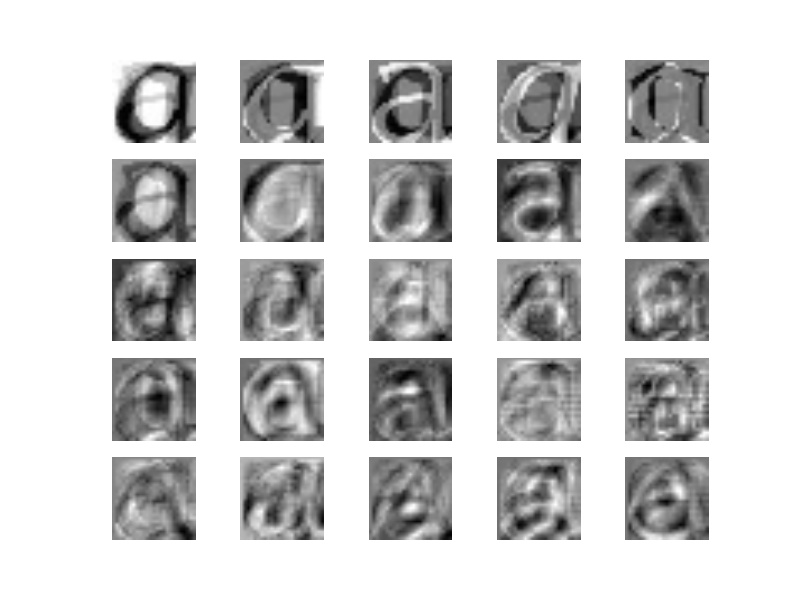
\includegraphics[scale=0.5]{display_save_25_comps.jpg}
    \caption{The first 25 principal components of the ``a"s. Generated using lines 154-155 and \texttt{display\_save\_25\_comps()}.}
    \label{fig:25a}
\end{figure*}
\begin{figure*}[h!]
    \centering
    
\includegraphics[scale=2]{immean.jpg}
    \caption{The mean image. Generated using line 154.}
    \label{fig:mean_a}
\end{figure*}

Interestingly, the mean image and the first principal component are extremely similar. Adding a scalar multiple of the first principal component would simply make the mean image darker or brighter. The principal components seem to be of the form ``emphasize one type of `a' while subtract another kind of `a'."

\textit{Advice: make observations about the output, and try to explain them.}

\end{homeworkProblem}
\clearpage
%----------------------------------------------------------------------------------------
%	PROBLEM 3
%----------------------------------------------------------------------------------------

\begin{homeworkProblem}
\noindent \textit{Reconstructing noiseless image using varying numbers of principal components.}

We reconstruct the noiseless image \texttt{1000\_t.jpg} using the first $N$ principal components, for various $N$. The quality of the reconstruction increases as $n$ increases. For just $1$ principal component, we simply get the mean image. For $25$ principal components, we are basically able to reconstruct the letter. The output for $100$ principal components is fairly close to perfect. The reconstruction is perfect when we use all $625$ principal components, as expected. (Note: $625 = 25\times 25$ is the dimensionality of the images.)

\textit{Advice: describe the quality of the results that you get. To the extent possible, explain why things are the way they are (e.g., why the reconstruction is perfect for $625$ components}.

\begin{figure*}[!ht]
\begin{subfigure}{.35\textwidth}
  
\includegraphics[width=.35\linewidth]{1pc.jpg}
  \caption{Reconstruction using \\1 principal component.}
  \label{fig:sfig1}
\end{subfigure}
\begin{subfigure}{.35\textwidth}
  
\includegraphics[width=.35\linewidth]{5pc.jpg}
  \caption{Reconstruction using \\5 principal components.}
  \label{fig:sfig2}
\end{subfigure}%
\begin{subfigure}{.35\textwidth}
  
\includegraphics[width=.35\linewidth]{25pc.jpg}
  \caption{Reconstruction using \\25 principal components.}
  \label{fig:sfig3}
\end{subfigure}
\begin{subfigure}{.35\textwidth}
  
\includegraphics[width=.35\linewidth]{100pc.jpg}
  \caption{Reconstruction using \\100 principal components.}
  \label{fig:sfig4}
\end{subfigure}%
\begin{subfigure}{.35\textwidth}
  
\includegraphics[width=.35\linewidth]{150pc.jpg}
  \caption{Reconstruction using \\150 principal components.}
  \label{fig:sfig5}
\end{subfigure}
\begin{subfigure}{.35\textwidth}
  
\includegraphics[width=.35\linewidth]{200pc.jpg}
  \caption{Reconstruction using \\200 principal components.}
  \label{fig:sfig6}%
\end{subfigure}
\begin{subfigure}{.35\textwidth}
  
\includegraphics[width=.35\linewidth]{400pc.jpg}
  \caption{Reconstruction using \\400 principal components.}
  \label{fig:sfig8}
\end{subfigure}
\begin{subfigure}{.35\textwidth}
  
\includegraphics[width=.35\linewidth]{all_pc.jpg}
  \caption{Reconstruction using \\all 625 principal components.}
  \label{fig:sfig11}
\end{subfigure}
\caption{}
\label{fig:pcs}
\end{figure*}

Figure~\ref{fig:pcs} demonstrates the effects of increasing the number of principal components.
These images were produced using the function \textbf{get\_reconstruction} (lines 65-70 and 158-164 of pca\_example.py).

\end{homeworkProblem}
\clearpage

%----------------------------------------------------------------------------------------
%	PROBLEM 4
%----------------------------------------------------------------------------------------

\begin{homeworkProblem}
\noindent \textit{Reconstructing images where salt-and-pepper noise was applied}

Noisy images are created using the function \texttt{salt\_and\_pepper\_noise()} (lines 98-106 of \texttt{pca\_example.py}). \\
The function \texttt{salt\_and\_pepper\_noise()} randomly sets a subselection of pixels to 0 or 1, while $noise\_prop$ is the proportion of the pixels set to either 0 or 1.
Once the salt-and-pepper noise is applied, the images are reconstructed using 200 principal components using the function 
\texttt{get\_reconstruction()} (lines 65-70 and 167-317 of \texttt{pca\_example.py}). 

We vary the proportion of pixels that are perturbed using salt-and-pepper-noise.

Some results are shown in  Figure~\ref{fig:a0all}, Figure~\ref{fig:a2all}, Figure~\ref{fig:a10all}, Figure~\ref{fig:a15all}.

For moderate amounts of noise, we are able to get a reconstruction that looks similar to the original image, without the noise.

After the proportion of pixels that are perturbed becomes greater than a certain threshold, (the threshold varies from one letter to another), the reconstruction gets worse and worse and eventually stops producing an image that looks like an 'a'.
The threshold in Figure~\ref{fig:a0all} and in Figure~\ref{fig:a10all} is around 60\% ($noise\_prop = 0.6$). 
That of Figure~\ref{fig:a2all} is around 45\% ($noise\_prop = 0.45$). 
Figure~\ref{fig:a15all} has the lowest threshold out of these four examples, at around 20\% ($noise\_prop = 0.2$).

\textit{Advice: look at the results, point out where the algorithm works, and where the algorithm doesn't work.}

\begin{figure*}[!ht]
\begin{subfigure}{.35\textwidth}
  \centering
  
\includegraphics[width=.35\linewidth]{a0reconstruction.jpg}
  \caption{Original image}
  \label{fig:a0}
\end{subfigure}%

\begin{subfigure}{.35\textwidth}
  \centering
  
\includegraphics[width=.35\linewidth]{a0noise0pt05.jpg}
  \caption{Image~\ref{fig:a0} with 5\% noise}
  \label{fig:a0noise0.05}
\end{subfigure}%
\begin{subfigure}{.35\textwidth}
  \centering
  
\includegraphics[width=.35\linewidth]{a0noise0pt05reconstruction200PCs.jpg}
  \caption{Reconstruction of Image~\ref{fig:a0noise0.05} using 200 principal components}
  \label{fig:a0noise0.05reconstruction}
\end{subfigure}%

\begin{subfigure}{.35\textwidth}
  \centering
  
\includegraphics[width=.35\linewidth]{a0noise0pt1.jpg}
  \caption{Image~\ref{fig:a0} with 10\% noise}
  \label{fig:a0noise0.1}
\end{subfigure}%
\begin{subfigure}{.35\textwidth}
  \centering
  
\includegraphics[width=.35\linewidth]{a0noise0pt1reconstruction200PCs.jpg}
  \caption{Reconstruction of Image~\ref{fig:a0noise0.1} using 200 principal components}
  \label{fig:a0noise0.1reconstruction}
\end{subfigure}%

\begin{subfigure}{.35\textwidth}
  \centering
  
\includegraphics[width=.35\linewidth]{a0noise0pt2.jpg}
  \caption{Image~\ref{fig:a0} with 20\% noise}
  \label{fig:a0noise0.2}
\end{subfigure}%
\begin{subfigure}{.35\textwidth}
  \centering
  
\includegraphics[width=.35\linewidth]{a0noise0pt2reconstruction200PCs.jpg}
  \caption{Reconstruction of Image~\ref{fig:a0noise0.2} using 200 principal components}
  \label{fig:a0noise0.2reconstruction}
\end{subfigure}%

\begin{subfigure}{.35\textwidth}
  \centering
  
\includegraphics[width=.35\linewidth]{a0noise0pt3.jpg}
  \caption{Image~\ref{fig:a0} with 30\% noise}
  \label{fig:a0noise0.3}
\end{subfigure}%
\begin{subfigure}{.35\textwidth}
  \centering
  
\includegraphics[width=.35\linewidth]{a0noise0pt3reconstruction200PCs.jpg}
  \caption{Reconstruction of Image~\ref{fig:a0noise0.3} using 200 principal components}
  \label{fig:a0noise0.3reconstruction}
\end{subfigure}%

\begin{subfigure}{.35\textwidth}
  \centering
  
\includegraphics[width=.35\linewidth]{a0noise0pt45.jpg}
  \caption{Image~\ref{fig:a0} with 45\% noise}
  \label{fig:a0noise0.45}
\end{subfigure}%
\begin{subfigure}{.35\textwidth}
  \centering
  
\includegraphics[width=.35\linewidth]{a0noise0pt45reconstruction200PCs.jpg}
  \caption{Reconstruction of Image~\ref{fig:a0noise0.45} using 200 principal components}
  \label{fig:a0noise0.45reconstruction}
\end{subfigure}%

\begin{subfigure}{.35\textwidth}
  \centering
  
\includegraphics[width=.35\linewidth]{a0noise0pt60.jpg}
  \caption{Image~\ref{fig:a0} with 60\% noise}
  \label{fig:a0noise0.60}
\end{subfigure}%
\begin{subfigure}{.35\textwidth}
  \centering
  
\includegraphics[width=.35\linewidth]{a0noise0pt60reconstruction200PCs.jpg}
  \caption{Reconstruction of Image~\ref{fig:a0noise0.60} using 200 principal components}
  \label{fig:a0noise0.60reconstruction}
\end{subfigure}%

\caption{}
\label{fig:a0all}
\end{figure*}

%%%%%%%%%%%%%%%%%%%%%%%%%%%%%%%%%%%%%%%%%%%%%%%%%%%%%%%%%%%%%%%%%%%%%%%

\begin{figure*}[!ht]
\begin{subfigure}{.35\textwidth}
  \centering
  
\includegraphics[width=.35\linewidth]{a2reconstruction.jpg}
  \caption{Original image}
  \label{fig:a2}
\end{subfigure}%15

\begin{subfigure}{.35\textwidth}
  \centering
  
\includegraphics[width=.35\linewidth]{a2noise0pt05.jpg}
  \caption{Image~\ref{fig:a2} with 5\% noise}
  \label{fig:a2noise0.05}
\end{subfigure}%
\begin{subfigure}{.35\textwidth}
  \centering
  
\includegraphics[width=.35\linewidth]{a2noise0pt05reconstruction200PCs.jpg}
  \caption{Reconstruction of Image~\ref{fig:a2noise0.05} using 200 principal components}
  \label{fig:a2noise0.05reconstruction}
\end{subfigure}%

\begin{subfigure}{.35\textwidth}
  \centering
  
\includegraphics[width=.35\linewidth]{a2noise0pt1.jpg}
  \caption{Image~\ref{fig:a2} with 10\% noise}
  \label{fig:a2noise0.1}
\end{subfigure}%
\begin{subfigure}{.35\textwidth}
  \centering
  
\includegraphics[width=.35\linewidth]{a2noise0pt1reconstruction200PCs.jpg}
  \caption{Reconstruction of Image~\ref{fig:a2noise0.1} using 200 principal components}
  \label{fig:a2noise0.1reconstruction}
\end{subfigure}%

\begin{subfigure}{.35\textwidth}
  \centering
  
\includegraphics[width=.35\linewidth]{a2noise0pt2.jpg}
  \caption{Image~\ref{fig:a2} with 20\% noise}
  \label{fig:a2noise0.2}
\end{subfigure}%
\begin{subfigure}{.35\textwidth}
  \centering
  
\includegraphics[width=.35\linewidth]{a2noise0pt2reconstruction200PCs.jpg}
  \caption{Reconstruction of Image~\ref{fig:a2noise0.2} using 200 principal components}
  \label{fig:a2noise0.2reconstruction}
\end{subfigure}%

\begin{subfigure}{.35\textwidth}
  \centering
  
\includegraphics[width=.35\linewidth]{a2noise0pt3.jpg}
  \caption{Image~\ref{fig:a2} with 30\% noise}
  \label{fig:a2noise0.3}
\end{subfigure}%
\begin{subfigure}{.35\textwidth}
  \centering
  
\includegraphics[width=.35\linewidth]{a2noise0pt3reconstruction200PCs.jpg}
  \caption{Reconstruction of Image~\ref{fig:a2noise0.3} using 200 principal components}
  \label{fig:a2noise0.3reconstruction}
\end{subfigure}%

\begin{subfigure}{.35\textwidth}
  \centering
  
\includegraphics[width=.35\linewidth]{a2noise0pt45.jpg}
  \caption{Image~\ref{fig:a2} with 45\% noise}
  \label{fig:a2noise0.45}
\end{subfigure}%
\begin{subfigure}{.35\textwidth}
  \centering
  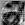
\includegraphics[width=.35\linewidth]{a2noise0pt45reconstruction200PCs.jpg}
  \caption{Reconstruction of Image~\ref{fig:a2noise0.45} using 200 principal components}
  \label{fig:a2noise0.45reconstruction}
\end{subfigure}%

\begin{subfigure}{.35\textwidth}
  \centering
  
\includegraphics[width=.35\linewidth]{a2noise0pt60.jpg}
  \caption{Image~\ref{fig:a2} with 60\% noise}
  \label{fig:a2noise0.60}
\end{subfigure}%
\begin{subfigure}{.35\textwidth}
  \centering
  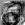
\includegraphics[width=.35\linewidth]{a2noise0pt60reconstruction200PCs.jpg}
  \caption{Reconstruction of Image~\ref{fig:a2noise0.60} using 200 principal components}
  \label{fig:a2noise0.60reconstruction}
\end{subfigure}%

\caption{}
\label{fig:a2all}
\end{figure*}

\begin{figure*}[!ht]
\begin{subfigure}{.35\textwidth}
  \centering
  
\includegraphics[width=.35\linewidth]{a10reconstruction.jpg}
  \caption{Original image}
  \label{fig:a10}
\end{subfigure}%

\begin{subfigure}{.35\textwidth}
  \centering
  
\includegraphics[width=.35\linewidth]{a10noise0pt05.jpg}
  \caption{Image~\ref{fig:a10} with 5\% noise}
  \label{fig:a10noise0.05}
\end{subfigure}%
\begin{subfigure}{.35\textwidth}
  \centering
  
\includegraphics[width=.35\linewidth]{a10noise0pt05reconstruction200PCs.jpg}
  \caption{Reconstruction of Image~\ref{fig:a10noise0.05} using 200 principal components}
  \label{fig:a10noise0.05reconstruction}
\end{subfigure}%

\begin{subfigure}{.35\textwidth}
  \centering
  
\includegraphics[width=.35\linewidth]{a10noise0pt1.jpg}
  \caption{Image~\ref{fig:a10} with 10\% noise}
  \label{fig:a10noise0.1}
\end{subfigure}%
\begin{subfigure}{.35\textwidth}
  \centering
  
\includegraphics[width=.35\linewidth]{a10noise0pt1reconstruction200PCs.jpg}
  \caption{Reconstruction of Image~\ref{fig:a10noise0.1} using 200 principal components}
  \label{fig:a10noise0.1reconstruction}
\end{subfigure}%

\begin{subfigure}{.35\textwidth}
  \centering
  
\includegraphics[width=.35\linewidth]{a10noise0pt2.jpg}
  \caption{Image~\ref{fig:a10} with 20\% noise}
  \label{fig:a10noise0.2}
\end{subfigure}%
\begin{subfigure}{.35\textwidth}
  \centering
  
\includegraphics[width=.35\linewidth]{a10noise0pt2reconstruction200PCs.jpg}
  \caption{Reconstruction of Image~\ref{fig:a10noise0.2} using 200 principal components}
  \label{fig:a10noise0.2reconstruction}
\end{subfigure}%

\begin{subfigure}{.35\textwidth}
  \centering
  
\includegraphics[width=.35\linewidth]{a10noise0pt3.jpg}
  \caption{Image~\ref{fig:a10} with 30\% noise}
  \label{fig:a10noise0.3}
\end{subfigure}%
\begin{subfigure}{.35\textwidth}
  \centering
  
\includegraphics[width=.35\linewidth]{a10noise0pt3reconstruction200PCs.jpg}
  \caption{Reconstruction of Image~\ref{fig:a10noise0.3} using 200 principal components}
  \label{fig:a10noise0.3reconstruction}
\end{subfigure}%

\begin{subfigure}{.35\textwidth}
  \centering
  
\includegraphics[width=.35\linewidth]{a10noise0pt45.jpg}
  \caption{Image~\ref{fig:a10} with 45\% noise}
  \label{fig:a10noise0.45}
\end{subfigure}%
\begin{subfigure}{.35\textwidth}
  \centering
  
\includegraphics[width=.35\linewidth]{a10noise0pt45reconstruction200PCs.jpg}
  \caption{Reconstruction of Image~\ref{fig:a10noise0.45} using 200 principal components}
  \label{fig:a10noise0.45reconstruction}
\end{subfigure}%

\begin{subfigure}{.35\textwidth}
  \centering
  
\includegraphics[width=.35\linewidth]{a10noise0pt60.jpg}
  \caption{Image~\ref{fig:a10} with 60\% noise}
  \label{fig:a10noise0.60}
\end{subfigure}%
\begin{subfigure}{.35\textwidth}
  \centering
  
\includegraphics[width=.35\linewidth]{a10noise0pt60reconstruction200PCs.jpg}
  \caption{Reconstruction of Image~\ref{fig:a10noise0.60} using 200 principal components}
  \label{fig:a10noise0.60reconstruction}
\end{subfigure}%

\caption{}
\label{fig:a10all}
\end{figure*}
%%%%%%%%%%%%%%%%%%%%%%%%%%%%%%%%%%%%%%%%%%%%%%%%%%%%%%%%%%%%%%%%%%%%%%%
\begin{figure*}[!ht]
\begin{subfigure}{.35\textwidth}
  \centering
  \includegraphics[width=.35\linewidth]{a15reconstruction.jpg}
  \caption{Original image}
  \label{fig:a15}
\end{subfigure}%15

\begin{subfigure}{.35\textwidth}
  \centering
  \includegraphics[width=.35\linewidth]{a15noise0pt05.jpg}
  \caption{Image~\ref{fig:a15} with 5\% noise}
  \label{fig:a15noise0.05}
\end{subfigure}%
\begin{subfigure}{.35\textwidth}
  \centering
  \includegraphics[width=.35\linewidth]{a15noise0pt05reconstruction200PCs.jpg}
  \caption{Reconstruction of Image~\ref{fig:a15noise0.05} using 200 principal components}
  \label{fig:a15noise0.05reconstruction}
\end{subfigure}%

\begin{subfigure}{.35\textwidth}
  \centering
  \includegraphics[width=.35\linewidth]{a15noise0pt1.jpg}
  \caption{Image~\ref{fig:a15} with 10\% noise}
  \label{fig:a15noise0.1}
\end{subfigure}%
\begin{subfigure}{.35\textwidth}
  \centering
  \includegraphics[width=.35\linewidth]{a15noise0pt1reconstruction200PCs.jpg}
  \caption{Reconstruction of Image~\ref{fig:a15noise0.1} using 200 principal components}
  \label{fig:a15noise0.1reconstruction}
\end{subfigure}%

\begin{subfigure}{.35\textwidth}
  \centering
  \includegraphics[width=.35\linewidth]{a15noise0pt2.jpg}
  \caption{Image~\ref{fig:a15} with 20\% noise}
  \label{fig:a15noise0.2}
\end{subfigure}%
\begin{subfigure}{.35\textwidth}
  \centering
  \includegraphics[width=.35\linewidth]{a15noise0pt2reconstruction200PCs.jpg}
  \caption{Reconstruction of Image~\ref{fig:a15noise0.2} using 200 principal components}
  \label{fig:a15noise0.2reconstruction}
\end{subfigure}%

\begin{subfigure}{.35\textwidth}
  \centering
  \includegraphics[width=.35\linewidth]{a15noise0pt3.jpg}
  \caption{Image~\ref{fig:a15} with 30\% noise}
  \label{fig:a15noise0.3}
\end{subfigure}%
\begin{subfigure}{.35\textwidth}
  \centering
  \includegraphics[width=.35\linewidth]{a15noise0pt3reconstruction200PCs.jpg}
  \caption{Reconstruction of Image~\ref{fig:a15noise0.3} using 200 principal components}
  \label{fig:a15noise0.3reconstruction}
\end{subfigure}%

\begin{subfigure}{.35\textwidth}
  \centering
  \includegraphics[width=.35\linewidth]{a15noise0pt45.jpg}
  \caption{Image~\ref{fig:a15} with 45\% noise}
  \label{fig:a15noise0.45}
\end{subfigure}%
\begin{subfigure}{.35\textwidth}
  \centering
  \includegraphics[width=.35\linewidth]{a15noise0pt45reconstruction200PCs.jpg}
  \caption{Reconstruction of Image~\ref{fig:a15noise0.45} using 200 principal components}
  \label{fig:a15noise0.45reconstruction}
\end{subfigure}%

\begin{subfigure}{.35\textwidth}
  \centering
  \includegraphics[width=.35\linewidth]{a15noise0pt60.jpg}
  \caption{Image~\ref{fig:a15} with 60\% noise}
  \label{fig:a15noise0.60}
\end{subfigure}%
\begin{subfigure}{.35\textwidth}
  \centering
  \includegraphics[width=.35\linewidth]{a15noise0pt60reconstruction200PCs.jpg}
  \caption{Reconstruction of Image~\ref{fig:a15noise0.60} using 200 principal components}
  \label{fig:a15noise0.60reconstruction}
\end{subfigure}%

\caption{}
\label{fig:a15all}
\end{figure*}

\end{homeworkProblem}
\clearpage

%----------------------------------------------------------------------------------------

\end{document}